\documentclass[]{IEEEtran}

% Your packages go here
\usepackage[utf8]{inputenc}
\usepackage{graphicx}
\usepackage{float}
\usepackage{listings}
\usepackage{xcolor}
%listings settings
\definecolor{codegreen}{rgb}{0,0.6,0}
\definecolor{codegray}{rgb}{0.5,0.5,0.5}
\definecolor{codepurple}{rgb}{0.58,0,0.82}
\definecolor{backcolour}{rgb}{0.95,0.95,0.92}
\definecolor{codeblue}{rgb}{0,0.8,0.99}
\definecolor{codeyellow}{rgb}{0.6,0.5,0}


\lstdefinestyle{vim_like}{
  backgroundcolor=\color{backcolour},   
  commentstyle=\color{codegreen},
  keywordstyle=\color{codeyellow},
  numberstyle=\tiny\color{codegray},
  stringstyle=\color{codepurple},
  basicstyle=\ttfamily\footnotesize,
  breakatwhitespace=false,         
  breaklines=true,                 
  captionpos=b,                    
  keepspaces=true,                 
  numbers=left,                    
  numbersep=5pt,                  
  showspaces=false,                
  showstringspaces=false,
  showtabs=false,                  
  tabsize=2
}
\lstset{style=vim_like}

\markboth{MO443 Digital Image Processing}{}

\begin{document}
  \title{Project 1 - Halftoning}
  \author{Thales Oliveira (RA 148051)
    \thanks{ra148051@students.ic.unicamp.br}
  }
  \maketitle
  
  \begin{abstract}

  \end{abstract}
  
\section{Introduction}
Halftoning is a technique which is used for reducing the number of colors used to represent an image, while is desired to keep a good visual perception of its contents for the user. In this work, the implementation of halftoning techniques with error diffusion was realized. For each technique, tests were executed to analyze the quality of the output image, sweeping the image in two different ways. The next section explains the implemented algorithms and the following, the tests done and the discussion.
\\
The code, along with the input files and the report is delivered in the compressed file THALES\_MATEUS\_RODRIGUES\_OLIVEIRA\_148051.tar, in the Google Classroom.
\section{The Program}
 
The program was implemented with Python 3.7.3. The libraries used and their respective versions are OpenCV 4.1.0 and Numpy 1.16.4.

\subsection{How to execute it}

The project has a Makefile available to help performing some actions on it. The Makefile has 3 basic instructions: clean, build and exec. Clean instruction removes generated images stored in the \textbf{output} folder, the source code in \textbf{bin} folder and the folders itself. The Build instruction creates the \textbf{output} and \textbf{bin} folders, and move execution code to \textbf{bin}. The Exec instruction executes the code with images in the \textbf{input} folder. Listing \ref{code:makefile} provides examples of how to execute the three instructions in a terminal.
\begin{lstlisting}[language=sh, caption={Makefile usage example}, label={code:makefile}]
  #clean environment, deletes output and bin folders and their content
  make clean
  
  #prepare the environment for code execution
  make build 

  #executes code
  make exec
\end{lstlisting}

\subsection{Input}

The program does not have an input argument by default, the input images are listed in code, and they are expected to be stored in the \textbf{input} folder. Listing \ref{code:input} shows how images are listed to be executed in code. The $images$ tuple is implemented in $src/main.py$

\begin{lstlisting}[language=Python, caption={Input images inside code}, label={code:input}]
  # for inserting other images, add tem to /input folder and list them here
  images = (
      'baboon',
      'monalisa',
      'peppers',
      'watch'
  )
\end{lstlisting}

\subsection{Output}
The output of the program is a series of halftoning images based on the input ones, changing the error diffusion methods and the sweeping directions. The output images are stored in the \textbf{output} folder, and the images are labeled by concatenating the image name, whether is colored or grayscale, the error diffusion method and the sweep order (\textit{e.g.: baboon\_colored\_sierra\_left-to-right.png})

\subsection{Implementation}
The function which implements the halftoning operation is defined in the \textit{src/halftoning.py} file. The file contains a dictionary that lists the approaches used for error diffusion, as mentioned in Figure 1 in the project proposal. Listing \ref{code:masks} shows the implemented dictionary.

\begin{lstlisting}[language=Python, caption={Masks used for error diffusion}, label={code:masks}]
  # Masks used for error propagation
  MASKS = {
      "floyd-steinberg": np.array([
        [0, 0, 7/16],
        [3/16, 5/16, 1/16]]),
      "stevenson-arce": np.array([
        [0, 0, 0, 0, 0, 32/200, 0],
        [12/200, 0, 26/200, 0, 30/200, 0, 16/200],
        [0, 12/200, 0, 26/200, 0, 12/200, 0],
        [5/200, 0, 12/200, 0, 12/200, 0, 5/200]]),
      "burkes": np.array([
        [0, 0, 0, 8/32, 4/32],
        [2/32, 4/32, 8/32, 4/32, 2/32]]),
      "sierra": np.array([
        [0, 0, 0, 5/32, 3/32],
        [2/32, 4/32, 5/32, 4/32, 2/32],
        [0, 2/32, 3/32, 2/32, 0]]),
      "stucki": np.array(
        [[0, 0, 0, 8/42, 4/42],
        [2/42, 4/42, 8/42, 4/42, 2/42],
        [1/42, 2/42, 4/42, 2/42, 1/42]]),
      "jarvis-judice-ninke": np.array([
        [0, 0, 0, 7/48, 5/48],
        [3/48, 5/48, 7/48, 5/48, 3/48],
        [1/48, 3/48, 5/48, 3/48, 1/48]])
  }
\end{lstlisting}
The function \textit{apply\_halftoning} implements the desired operation. It receives the original image, the name of the error diffusion approach, the sweep method (left to right or alternated), and a benchmarking flag to monitor execution time. Listing \ref{code:halftoning} shows keyparts of implementation

\begin{lstlisting}[language=Python, caption={Implementation of halftoning solution}, label={code:halftoning}]
def apply_halftoning(img, err_method="floyd-steinberg", sweep_method=1, benchmarking=False):
  # initialize result array
  result = np.zeros_like(img)
  # separates the masks that could be used
  # (it needs the flip version of mask for alternated sweep)
  m = (0, MASKS[err_method], np.flip(MASKS[err_method], 1))
  # saves mask dimensions to be used when needed
  mask_h, mask_w = m[1].shape
  # saves image dimensions to be used when needed
  img_h, img_w = img.shape
  # it holds the offset of manipulated pixel related to mask
  offset = mask_w//2
  # applies padding to image to make it easier the operations with mask
  img_padded = np.pad(img, ((0, mask_h - 1), (mask_w//2, mask_w//2)), 'constant')

  # default starting direction (left to right)
  direction = 1
  # default index values for sweeping from left to right and right to left
  sweep_options = (0, (0, img_w), (img_w - 1, 0))

  # it sweeps the image from top to bottom
  for j in range(img_h):
      # it sweeps the image from left to right or right to left depending on direction
      beginning, end = sweep_options[direction]
      # do the horizontal sweeping
      for i in range(beginning, end, direction):
          # depending on analyzed pixel, set its result value according to threshold
          if img_padded[j][(i + offset)] < 128:
              result[j][i] = 0
          else:
              result[j][i] = 1

          # calculates associated error
          error = img_padded[j][(i + offset)] - result[j][i]*255
          # propagates error according to mask
          img_padded[j:j+mask_h, i:i+mask_w] = (img_padded[j:j+mask_h, i:i+mask_w]
                                                + (error*m[direction])).astype(np.uint8)
      # it changes from left to right to right to left (vice-versa) depending on the sweep method
      direction *= sweep_method

  # scale the result
  return result*255

\end{lstlisting}
The decisions made in the implementation are explained in the following part.
\subsubsection{Dealing with sweeping directions}
In this solution, it was implemented two approaches: sweeping every line from left to right, and alternating directions when changing from one line to the other. Figure \ref{fig:sweepingmodes} shows the approaches. If the second mentioned method is chosen, the error diffusion mask has to be mirroed in the vertical direction. In other to avoid \textit{if-else} statements when deciding whether mask to use for the specific line (the regular or the mirroed one), the tuple \textit{m} holds both masks, and decide which one to use based on the \textit{direction} flag (if \textit{direction} is 1, use the regular mask. If it is -1, use the mirroed one). To sweep the image from right to left, it is also considered the indexes in the loop to decrease. Following the same idea of tuple \textit{m}, the tuple \textit{sweep\_options} is used to set the starting index, the stop index, and the \textit{direction} flag as step.

\begin{figure}[H]
  \centering
  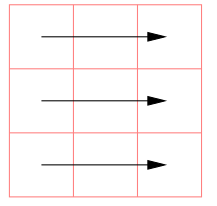
\includegraphics[width=0.4\hsize]{images/sw-left-to-right.png}
  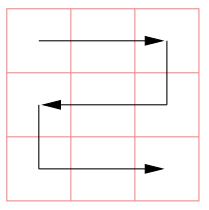
\includegraphics[width=0.4\hsize]{images/sw-alternate.png}
  \label{fig:sweepingmodes}
  \caption{Left: Sweeping from left to right. Right: Sweeping alternated}
\end{figure}

\subsubsection{Image Padding to deal with borders}
In order to deal with pixels in the border of the image, to diffuse the error, the image is padded as the mask propagates the error to its neighbors, as they may not exist for pixels in the border. The padding is done based on the mask properties, such as not diffusing errors to already visited pixels and the dimensions of each mask. The values padded does not matter, as they are not visited.

\subsubsection{Defining the value of the pixel and the error diffusion}
The main ideia of the halftoning algorithm is the following: rather than a simple binarization, in order to create the "feeling" of having more than 2 intensities of a color in the image, an analyzed pixel propagates its information to specific close neighbors. This propagation of information is what we define as error diffusion. Based on a threshold which defines whether a pixel has the maximum or minimum intensity, the resulting pixel value is defined and the error is calculates and passed through specific neighbors with specific weights. That weight is what is defined in the error diffusion masks. The error diffused for the neighbor pixels is proportional to the mentioned weight. After performing these steps to all pixels in the image, the process is done. The steps are the ones inside the two \textit{for} statements in listing \ref{code:halftoning}. They were implemented based on Algorithm 5, presented on the \textit{Enhancement} class of MO443: Introduction to Digital Image Processing course.  

\subsubsection{Sweeping the image}
To perform the visit of every pixel, as seen in listing \ref{code:halftoning}, it is used 2 nested \textit{for} statements. As the author was unable to vectorize the error propagation, the execution time occours in the second scale. To defined the value of the analyzed pixel in the iteration, an  offset is used, as the 

%  \begin{lstlisting}[language=Python, caption={Nearest neighbor interpolation function.}, label={code:nninterpolation}]
% def resize(img, shape):
%     ...
%     # build the new image with shape intended
%     result = np.zeros(shape[0]*shape[1]*3).reshape(shape[0], shape[1], 3)

%     # get y and x ratios to calculate pixels positions to take
%     y_ratio = shape[0]/img.shape[0]
%     x_ratio = shape[1]/img.shape[1]

%     for y in range(shape[0]):
%         for x in range(shape[1]):
%             result[y,x] = img[int(y/y_ratio),int(x/x_ratio)]

%     return result.astype(np.uint8)
% \end{lstlisting}

% \begin{figure}[H]
%     \centering
%     \includegraphics[width=0.4\hsize]{img/o-cv2-a.png}
%     \includegraphics[width=0.4\hsize]{img/o-nninterpo-a.png}
%     \includegraphics[width=0.4\hsize]{img/o-cv2-b.png}
%     \includegraphics[width=0.4\hsize]{img/o-nninterpo-b.png}
%     \caption{Image results from resizing. Left images: 30x30 and 700x700 images reduced with OpenCV's cubic interpolation. Right images: 30x30 and 700x700 images reduced with our nearest neighbor and Gaussian blur approach}
%     \label{fig:resize-compare}
% \end{figure}

% \begin{table}[h!]
% \centering
% \begin{center}
% \begin{tabular}{ |c|c| } 
%  \hline
%  Alphabets & Description \\
%  \hline
%  {[}'\#', '@', '\%', '=', '*', ':', '-', '.', ' '{]} & Default (required) \\ 
%  \hline
%  {[}'W', 'B', 'H', 'T', 'L', 'I', '.', ' '{]}  & Uppercase letters  \\
%  \hline
%  {[}'8', '6', '2', '1', '+', '-', '.', ' '{]} & Mathematical  \\ 
%  \hline
%  ['\}', ']', '|', '!', '"', ':', '.', ' '] & Vertical \\
%  \hline
%  ['\#', '=', '"', '\~','-', '\_', '.', ' '] & Horizontal \\
%  \hline
% \end{tabular}
%  \label{table:alphabet}
%  \caption{Alphabets used in experiments}
% \end{center}
% \end{table}

\section{Experiments}

\section{Discussion}

\section{Conclusion}


\end{document}
